\section{Multi-Agent Systems}
\label{sec:multi-agent}

A single LLM-based agent, built as in Section~\ref{sec:agent-anatomy}, has limits that grow with the difficulty of the task. Its short-term memory is the information inside the context window, and the transformer architecture bounds it \cite{wangSurveyLargeLanguage2024}. Multi-agent orchestration answers this with a paradigm in which specialized agents assume distinct roles, exchange information through structured protocols, and coordinate their actions to solve problems beyond the reach of any single agent \cite{zhuLLMBasedMultiAgentOrchestration2026a}. Compared with a system that uses a single LLM-based agent, this paradigm specializes LLMs into distinct agents, each with different capabilities, that interact with each other \cite{guoLargeLanguageModel2024}. Section~\ref{sec:coordinator} examines the coordinator-based routing pattern this work studies, in which a coordinator assigns each query to a specialized agent.

Zhu et al. defined the \emph{coordination topology} of a multi-agent system as the directed graph whose vertices are the agents and whose edges are the message-passing or delegation pathways declared at design time \cite{zhuLLMBasedMultiAgentOrchestration2026a}. This graph expresses which agent may direct another, and along which paths messages flow between agents. Their taxonomy has three topologies: centralized, where the graph is a star with a designated supervisor; decentralized, where it is a peer graph with no designated supervisor; and hierarchical, where it is a tree \cite{zhuLLMBasedMultiAgentOrchestration2026a}.

A second axis of the same taxonomy is runtime adaptivity. Here, the active edges are the subset of the topology's edges that carry a message at a given step, distinct from the full edge set declared at design time. A system is static when its vertices, its active edges, and its routing policy are fixed at design time and do not change for the duration of a task, and dynamic-adaptive when that configuration changes at run time, for instance when only the active edge subset changes while the vertices and the permitted edges stay fixed \cite{zhuLLMBasedMultiAgentOrchestration2026a}. The axis is orthogonal to the topology, so any of the three topologies can be static or dynamic-adaptive \cite{zhuLLMBasedMultiAgentOrchestration2026a}.

\subsection{Centralized}
\label{subsec:topology-centralized}

A single supervisor agent owns the workflow: it decomposes the incoming task, assigns subtasks to worker agents, collects their outputs, and decides what happens next \cite{zhuLLMBasedMultiAgentOrchestration2026a}. Every message passes through the supervisor, which therefore keeps a global view of the progress of the task, and the supervisor is typically a language model that reads the current state to select the next worker \cite{zhuLLMBasedMultiAgentOrchestration2026a}. Guo et al. described the same shape as centralized communication, where a central agent coordinates the communication of the system and the other agents interact through this central node \cite{guoLargeLanguageModel2024}. The supervisor is also a single point of failure and a throughput bottleneck, and its context window fills as the number of agents and the length of the conversation grow, which makes the topology suitable for a modest number of agents, roughly three to seven \cite{zhuLLMBasedMultiAgentOrchestration2026a}.

\begin{figure}[ht]
	\centering
	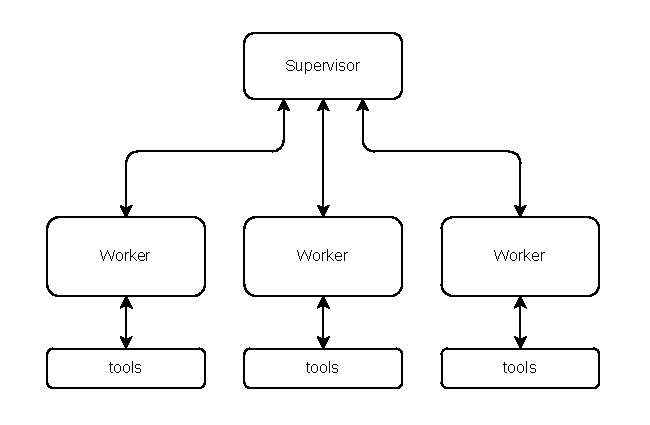
\includegraphics[width=0.72\textwidth]{images/topology_centralized.pdf}
	\caption[Centralized topology]{Centralized topology}
	\label{fig:topology-centralized}
\end{figure}

\subsection{Decentralized}
\label{subsec:topology-decentralized}

No central coordinator exists. The agents communicate directly, and each one decides on its own when to act, whom to consult, and how to contribute. Task allocation emerges from negotiation and self-selection, with each agent holding local state and taking its own routing decisions \cite{zhuLLMBasedMultiAgentOrchestration2026a}. Guo et al. described the same shape as decentralized communication, which operates on a peer-to-peer network where agents communicate directly with each other \cite{guoLargeLanguageModel2024}. They called the corresponding interaction style the debate paradigm, where agents present and defend their own viewpoints or solutions and criticize those of the others to reach a consensus or a more refined solution \cite{guoLargeLanguageModel2024}. The topology removes the single point of failure and lets solutions emerge from unconstrained interaction, but coherent global behavior is hard to guarantee and distributed execution traces make later debugging laborious \cite{zhuLLMBasedMultiAgentOrchestration2026a}. The absence of a single control point also places this topology outside the scope of the routing pattern this work studies, since there is no vertex at which a coordination decision of the kind defined in Section~\ref{sec:coordinator} could be located.

\begin{figure}[ht]
	\centering
	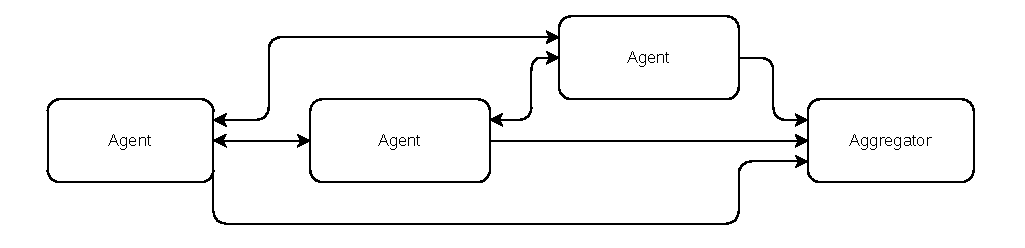
\includegraphics[width=0.88\textwidth]{images/topology_decentralized.pdf}
	\caption[Decentralized topology]{Decentralized topology}
	\label{fig:topology-decentralized}
\end{figure}

\subsection{Hierarchical}
\label{subsec:topology-hierarchical}

The agents are organized in a tree. Manager agents assign subtasks to the level below, and results return to the level above; this is assignment as defined in Section~\ref{sec:coordinator}, since a manager continues the work once its subordinate reports back. Each manager covers one domain or subtask scope and may decompose its assignment further, so top-level managers assign subtasks to mid-level managers and these assign subtasks to leaf-level workers \cite{zhuLLMBasedMultiAgentOrchestration2026a}. An agent that is a worker for its parent is therefore a manager for its own children, and the decision taken once by the supervisor of Figure~\ref{fig:topology-centralized} is repeated at every internal node. Communication scales linearly within the tree rather than quadratically across the full set of agents. This suits large decomposable tasks and systems that must grow beyond ten to fifteen agents, at the cost of the latency of multi-level message passing \cite{zhuLLMBasedMultiAgentOrchestration2026a}. Intermediate managers also become bottlenecks when the tree is not balanced \cite{zhuLLMBasedMultiAgentOrchestration2026a}. Guo et al. described the same shape as layered communication, where agents at each level have distinct roles and interact within their layer or with adjacent layers \cite{guoLargeLanguageModel2024}. Magentic-One extends the pattern with a lead orchestrator that plans, tracks progress, and replans to recover from errors, directing specialized agents for web browsing, file navigation, and code execution \cite{zhuLLMBasedMultiAgentOrchestration2026a}.

\begin{figure}[ht]
	\centering
	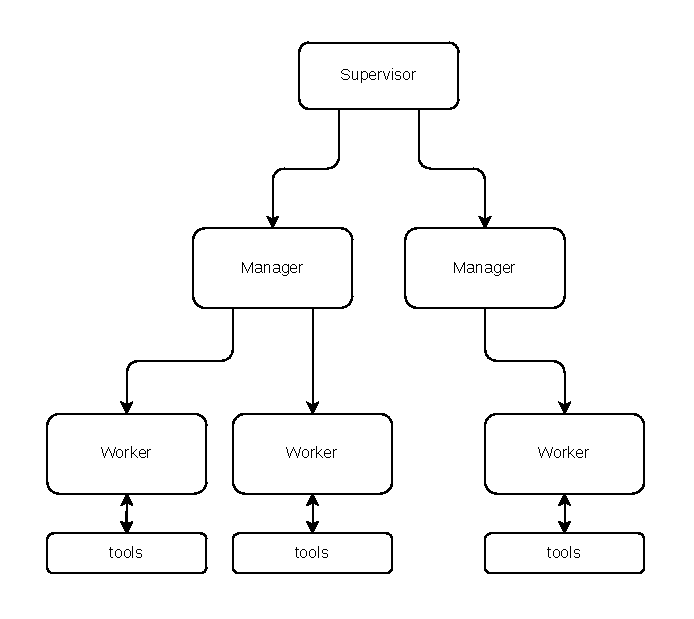
\includegraphics[width=0.7\textwidth]{images/topology_hierarchical.pdf}
	\caption[Hierarchical topology]{Hierarchical topology}
	\label{fig:topology-hierarchical}
\end{figure}



\subsection{Orchestration frameworks}
\label{subsec:topology-frameworks}

These topologies are not merely descriptive categories: they are the constructs that current frameworks expose. Zhu et al. observed that, without a dedicated orchestration layer, agents show three canonical failure modes:
\begin{itemize}
	\item task duplication, where several agents solve the same subtask independently;
	\item contradictory outputs, where agents produce inconsistent artifacts from shared premises;
	\item convergence failure, where the system cycles indefinitely without reaching a terminal state \cite{zhuLLMBasedMultiAgentOrchestration2026a}.
\end{itemize}
The frequency and the severity of these failures increase with the number of agents and the complexity of the task, which is why Zhu et al. treated orchestration as a first-class engineering concern and not as an implementation afterthought \cite{zhuLLMBasedMultiAgentOrchestration2026a}. Every major framework exposes configuration options for it, in the form of speaker-selection policies, delegation flags, conditional edges, and manager swaps. Most frameworks are therefore not restricted to a single cell of the taxonomy and instead cover a small contiguous region of it, with one primary cell obtained from the documented defaults and adjacent cells reachable through configuration \cite{zhuLLMBasedMultiAgentOrchestration2026a}.
